\section{Framework Overview} \label{framework}
In this section, 
% we propose our novel fully homomorphic database framework, 
% called \NAME,
% to query and process encrypted data with  
% cost-effectiveness, high elasticity, and high security.
we first provide a high-level workflow 
of \NAME in \cref{framework:workflow},
and then analyze the threat model and security guarantees of \NAME
in \cref{framework: threat_model}. Lastly, we summarize how to
implement key SQL statements for the filter-aggregation process
in \cref{block: overview}.

% briefly review the overall workflow 
% and 
% the overall architecture
% and then provide a straightforward example to illustrate the \NAME workflow.


\subsection{\NAME Workflow} \label{framework:workflow}
\begin{figure*}[t!]
   \begin{center}
   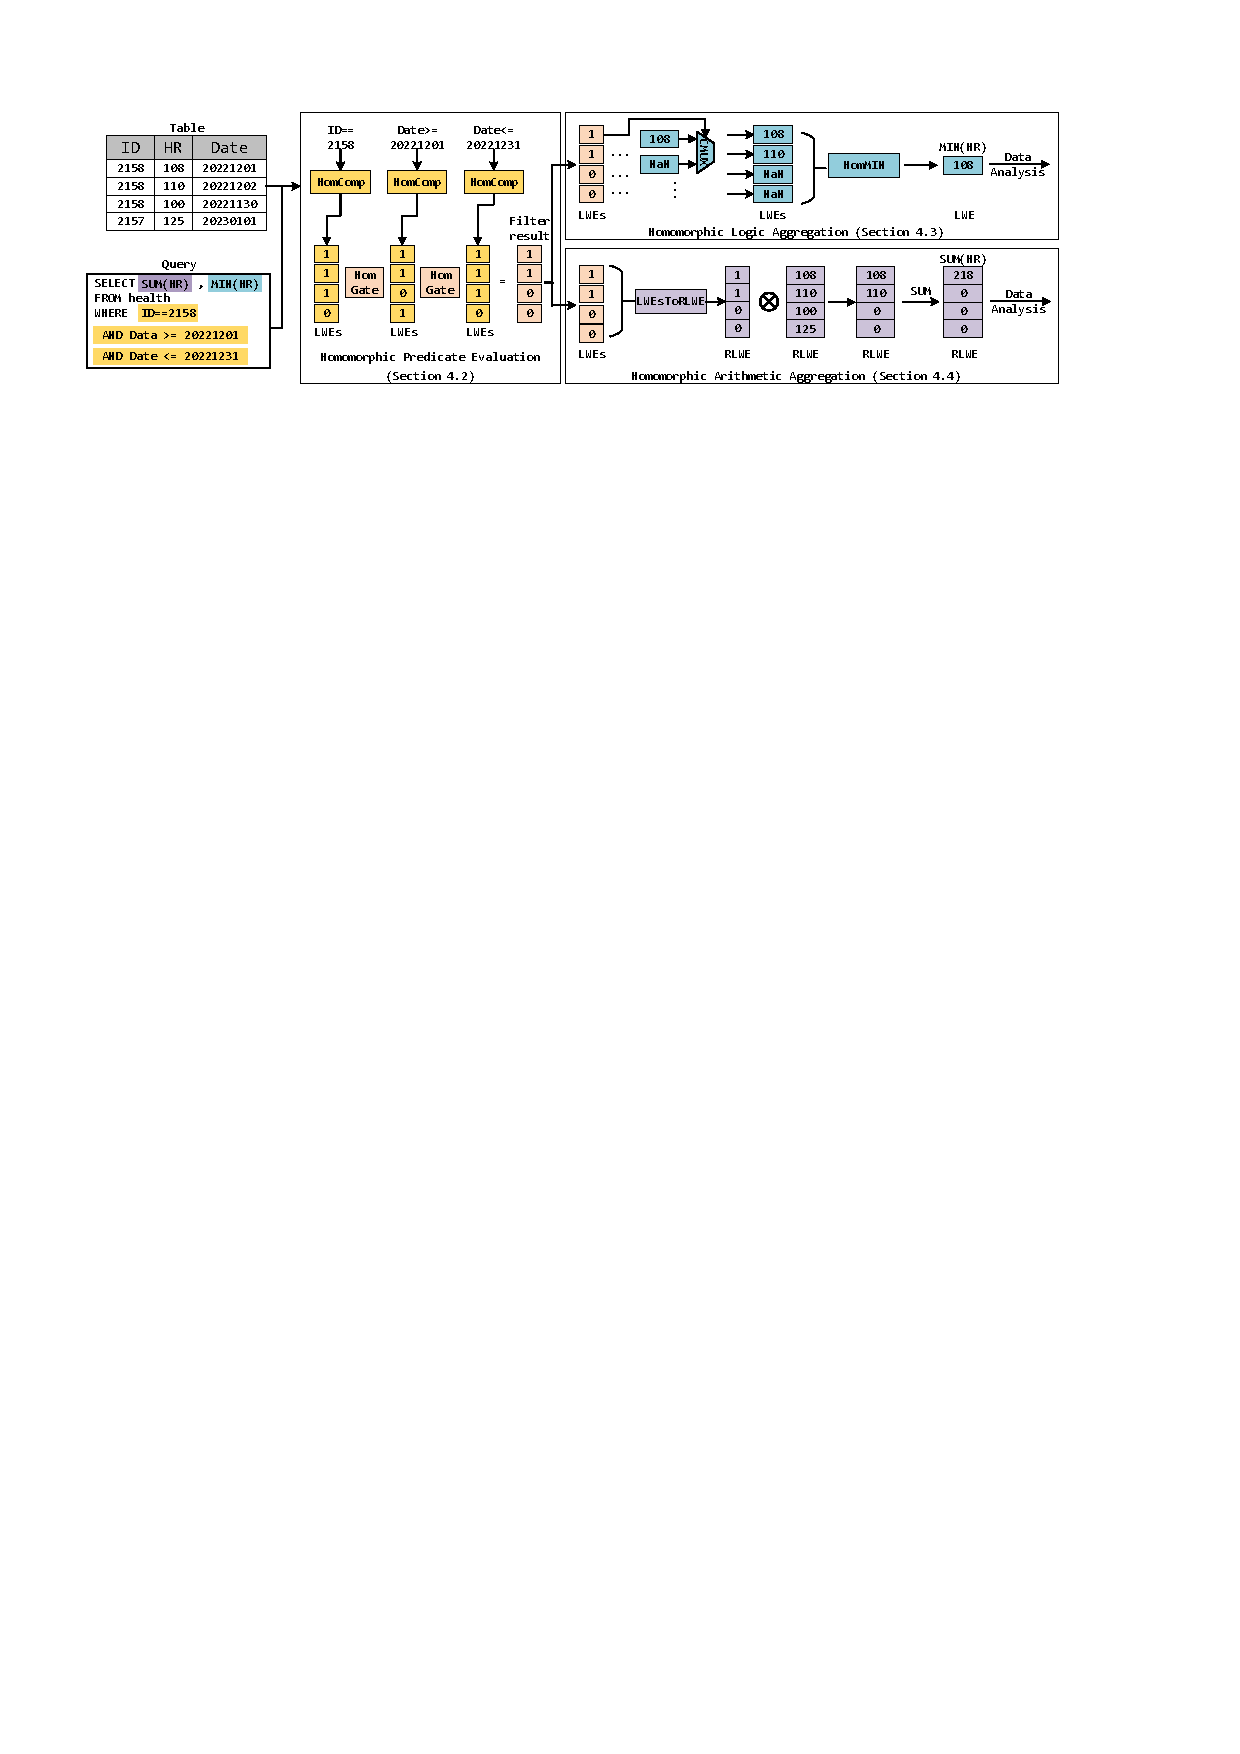
\includegraphics[width=\linewidth]{figure/query_evaluation.pdf}
   \end{center}
    % \vspace{-0.5em}
      \caption{An example processing
      flow illustration in query evaluation. Here, we show
      how to perform logic aggregation ($\hommin$) and arithmetic aggregations.
      Plaintext values in the figure are used only to demonstrate
      the range for each of the attributes.}
      \Description{A encrypted query evaluation process consists of three parts: 
      homomorphic predicate evaluation, homomorphic logic aggregation, and homomorphic
      arithmetic aggregation.}
   \label{fig: query_eva}
   % \vspace{-0.5em}
\end{figure*}
\begin{table*}[t!]
    % \footnotesize
    \centering
    \caption{Summary of Operation Costs for Each Homomorphic SQL 
    Statement.}

    % \vspace{-0.5em}
        \begin{tabular}{ccccc}
            \toprule
            SQL Statement & \#\homcomp & \#\homgate & \#\cmux & \#\cb\\
            \midrule
            $\select$ & $\dbtabrow \cdot \dbabsquery$& 
            $\dbtabrowsize \cdot (\dbabsquery - 1)$ & 0 & 0\\
            $\join$ & $\abs{\dbtab_a}_{\rm row} \cdot \abs{\dbtab_b}_{\rm row}$&
            0 & 0 & 0\\
            $\groupby$ & $\dbtabrow \cdot \abs{\attribute}$ &
            0 & 0 & 0\\
            $\orderby$ & $\dbtabrow \log_{2}^{2}{\dbtabrow } $ & 0 
            & $\dbtabrow (\log_{2}^{2}{\dbtabrow } + 1) $&
            $\dbtabrow (\log_{2}^{2}{\dbtabrow } + 1) $ \\
             $\dbmin/\dbmax$ & $\dbtabrow - 1$ & 0 & $2\dbtabrow - 1$ & $2\dbtabrow - 1$\\
            
            
            \bottomrule
        \end{tabular}\\
    \label{tab: sqlcost}
    {\footnotesize{$|\dbquery|, \dbtabrowsize$ and
    $|\attribute|$ are all public data known to the server.}}
\end{table*}
The \NAME framework is composed of three interlinked stages:
%as depicted in \cref{fig: workflow}: 
(1) offline data encryption, 
(2) online query processing, and (3) online data analysis.
In what follows, we detail the main objective of each stage and 
briefly sketch the lower-level FHE operations.

% \begin{figure*}[t!]
%     \begin{tabular}{p{0.2cm}<{\raggedright}
%     m{7cm}<{\raggedright}
%     m{2cm}<{\centering}
%     m{6.5cm}<{\raggedright}}
%     \toprule
%     & \multicolumn{1}{c}{Client} & &  \multicolumn{1}{c}{Server} \\
%     \midrule
%     \multicolumn{2}{l}{{\bf{Offline Data Encryption Stage}}} & & \\
%     1.& Set up FHE parameters and secret key. & & \\
%     2.& Initialize data $\mathcal{T} = (t_1, t_2, ..., t_{\abs{\mathcal{T}}_c})$ & &\\
%     3.& Initialize Model: $\mathcal{M} = (w_{1}, w_{2}, ..., w_{\lvert \mathcal{M} \rvert_c}, 
%     \mathcal{C})$ & & \\
%     4. & Encrypts each column of $\mathcal{T}$ using RLWE encryption
%     and gets the encrypted table: $\mathcal{CT} = 
%     (ct_1, ct_2, ..., ct_{\lvert \mathcal{T} \rvert_c})$ & 
%     $\xrightarrow{\quad\mathcal{CT}\quad}$  & Encrypted Table: $\mathcal{CT}$ \\
%     5.& Encrypts each weight of the model and
%     gets the encrypted model $\mathcal{CM} =
%     = (cw_1, cw_2, ...,cw_{\lvert \mathcal{M} \rvert_c}, \mathcal{C})$ &
%     $\xrightarrow{\quad\mathcal{CM}\quad}$ & Encrypted Model: $\mathcal{CM}$ \\
%     \midrule
%     \multicolumn{2}{l}{{\bf{Online Query Processing Stage}}} & & \\
%     4.& Initialize Query: $\mathcal{Q} = (p_{1}, p_{2}, ..., p_{\abs{\mathcal{Q}}}, B, G)$ & & \\
%     5.& Encrypts each predicate of the query and gets the encrypted query
%     $\mathcal{CQ} = 
%     (cp_{1}, cp_{2}, ..., cp_{\abs{\mathcal{Q}}}, B, G)$ & 
%     $\xrightarrow{\quad\mathcal{CQ}\quad}$ & 
%     Encrypted Query: $\mathcal{CQ}$ \\
%     6.& & & Processing $\mathcal{CQ}$ 
%     on $\mathcal{CT}$ 
%     and gets the encrypted query result 
%     $\mathcal{CR} = (cr_1, cr_2,..., cr_{\abs{G}})$ \\
%     \midrule
%     \multicolumn{2}{l}{{\bf{Online Data Analysis Stage}}} & & \\
%     10.& & & Switch the query result for data analysis
%     and gets the analysis result: $ \mathcal{CR}_{\mathcal{M}}=\mathcal{CM}(\mathcal{CR})$ \\
%     11.& Decrypts and gets the final result: $\mathcal{M}(\mathcal{R})$ & 
%     $\xleftarrow{\quad\mathcal{CR_{\mathcal{M}}}\quad}$ & Evaluation Result:  $\mathcal{CR}_{\mathcal{M}}$\\
%     \bottomrule
%     \end{tabular}
%     \caption{The workflow illustration of \NAME with three main stages: the offline data encryption stage, the online query processing stage, and the 
%     online data analysis stage. }
%     %The notation follows the definition in \cref{pre: he_db}}
%     \label{fig: workflow}
% \end{figure*}

% \textbf{(1) Offline Data Encryption Stage}: 

To begin with,  in (1) the offline data encryption stage, 
the client first needs to encrypt all the data tables in the database 
using FHE and outsources the encrypted database to the server. 
Specifically, for every table $\dbtab\in\db$, each column $t_i\in\dbtab$ 
will first be divided into $J=\lceil \dbtabrowsize/N\rceil$ data chunks,
each of size $N$. Next, 
each data chunk is encoded into a degree-$N$ plaintext polynomial $\ttm_{i, j}$, and 
encrypted into an RLWE ciphertext $\rlwe(\ttm_{i, j})$. The resulting encrypted
database is thus a set of RLWE ciphertexts $\{\rlwe(\ttm_{i, j})\}$ along
with the associated keys (i.e., $\bBK$ and $\mathbf{CK}$).
Along with the encryption database, the evaluation keys $\bBK$
will also be sent to the server.
We note that different from existing bit-by-bit~\cite{aphadb}
and row-by-row~\cite{heda} schemes, we encrypt the entire database using only RLWE
ciphertexts, significantly reducing the client-side encryption complexity and communication
burdens.
% Based on the security of the FHE ciphertexts, 
% the server could not gain any information without 
% the secret key. 
% We provide more security analysis in \cref{framework: threat_model}.


% \textbf{(2) Online Query Processing Stage}:
Next, two main steps in (2) the online query processing stage,
are homomorphic filtering and homomorphic aggregation. 
% Here, the client initiate SQL query over the outsourced data, 
% which can contain a set of particular combination of the 
% $\select$, $\join$, $\groupby$, $\orderby$, aggregation and further data analysis 
% operations. 
For filtering, we execute a number of homomorphic comparisons to
realize the $\select$, $\join$, $\groupby$, and $\orderby$ filtering 
operations on
encrypted data items, and more details on the exact input-output
behaviors of these SQL statements are provided in \cref{block: overview}. 
Then, logic 
(\texttt{MIN}, \texttt{MAX}, \texttt{Top-k})
and arithmetic (\texttt{SUM}, \texttt{AVG}) aggregations are executed
according to the statements in the queries. To better convey our idea,
we first summarize how the SQL statements are built over the proposed FHE 
operators in \cref{block: overview}. Later in \cref{block},
the proposed high-precision homomorphic comparison, aggregation,
and conversion operators are presented. % can be found in \cref{block}.
% We point out two
% main challenges here. First, it is highly non-trivial to
% efficiently evaluate a rich class of encrypted predicates with
% unbounded predicate depth and high operand precision.
% cost-effectiveness and high precision (\cref{block: comparison}).
% The server evaluates the query $\mathcal{CQ}$ 
% on the encrypted table $\mathcal{CT}$
% homomorphically.
% The processing of the encrypted query on encrypted data follows two steps: 
% The filtering period retrieves records from the table 
% according to the specified predicate from the clause,
% which contains lots of comparisons 
% as well as logic gates.
% The aggregation stage groups multiple values of 
% filtering results to 
% calculate a summary value, which consists of logical aggregations

% Although FHE could support these operations nat\"ively, 
% there still faces two main challenges. 
% The first is how to perform unbounded encrypted predicate evaluation with
% cost-effectiveness and high precision (\cref{block: comparison}).
% As the filtered result is in encrypted form, the second challenge is 
% how to evaluate homomorphic aggregations
% only on filtered rows with high precision, 
% including homomorphic logic aggregations (\cref{block: minmax})
% and homomorphic arithmetic aggregations (\cref{block: LWEsPack}).


% While the user is willing to query her data, 
% she encrypts the sensitive part (predicate value) of the query
% and sends the homomorphically encrypted query $\mathcal{CQ}$
% to the cloud server.


% \textbf{(3) Online Data Analysis}: 
If needed, the server performs further computations on 
the aggregated results in (3), the online data analysis stage.
In most practical applications, the client 
also wishes to outsource some data analysis 
algorithms. Here, we assume that
%To achieve such a goal, the user encrypts the model and sends it to the server.
the data analysis algorithm $\calgo$ contains a set of algorithm parameters  $\algoweight$,
which belongs to either the client or the server.
Unfortunately, due to the limit of 
ciphertext noise level~\cite{aphadb, heda} or incompatible plaintext encoding~\cite{sagma},
queried results produced by existing FHE-based SDO often cannot be further 
processed without additional client-server interactions.
In contrast, through the carefully designed homomorphic aggregation and conversion operators,
\NAME permits arbitrary $\calgo$ to be applied on the queried ciphertext results.
A detailed presentation for the data analysis stage can be found in \cref{Analysis}.
% data analysis methods may not achieve the best efficiency
% when dealing with aggregation results obtained from step \textbf{(2)},
% due to the unmatched ciphertext formats~\cite{sagma} or noise overflow~\cite{aphadb, heda}.
% Though, it is necessary to switch (\revise{bootstrap}) the aggregated ciphertext elastically 
% to support general data analysis (\cref{Analysis}). 

\subsection{Threat Model and Security} \label{framework: threat_model}
{\bf{Threat Model}}: Our security goal is to protect the outsourced database $\mathcal{D}$
owned by the client $\mathcal{C}$ from the semi-honest server $\mathcal{S}$,
and our threat model is similar to that in previous works\cite{cryptdb, sagma, aphadb, 
sortinghat, heda}.
% Here, the $\mathcal{C}$ encrypts the private $\mathcal{D}$
% using FHE and outsources to the $\mathcal{S}$. 
We assume that $\mathcal{S}$ honestly follows the protocol to
execute the queries and data analysis algorithms, but acts as 
a probabilistic polynomial time adversary and perform computations to 
learn as much as possible from $\db$ owned by $\mathcal{C}$.
The concrete public and private data from the perspective of the server is as follows. 
% the notation follows the definition in \cref{pre: he_db}.

\noindent {\bf{Public Data}}: 
\begin{itemize}
    \item $\abs{\mathcal{D}}$:
    the size of the database, i.e., the number of data tables in $\mathcal{D}$.
    \item $\dbtabrowsize$, $\dbtabcolsize$:
    the number of rows as well as the number of columns in some
    table $\dbtab\in\db$. 
    \item $\abs{\dbquery}$: 
    the number of filtering predicates in a SQL query $\dbquery$.
    \item $\attribute, |\attribute|$: The attribute label (e.g., gender, date)
    and the range of the attribute (e.g., $|\mathsf{Gender}|=2$).
    \item The logic connection (e.g., AND, OR) between the filtering predicates in a SQL query.
    \item The aggregation functions (e.g., $\dbsum$, $\dbmin$) in a SQL query. 
    \item $\calgo$: the data analysis algorithm without parameters (i.e., only the procedures).
\end{itemize}

\noindent {\bf{Private Data}}: %The following data need to be protected from the server.
\begin{itemize}
    \item $\mathcal{T}_{i, j}$,
    for $i \in \dbtabrowsize$, $j \in \dbtabcolsize$
    : exact values of the database items for all $\dbtab\in\db$.% i.e.,  
    \item $\mathcal{Q}_i \in \mathcal{Q}$, for $i \in \abs{\mathcal{Q}}$: 
    the predicate values in the SQL query.
    \item $w_i \in \mathcal{W}$, for $i \in \abs{\mathcal{W}}$: 
    the weight values of the data analysis algorithm $\calgo$.
\end{itemize}

{\bf{Security of \NAME}}: Since the private data are all encrypted using
FHE, the security of \NAME can be directly 
reduced to that of the underlying FHE scheme.
Traditional FHE schemes, such as B/FV~\cite{DBLP:conf/crypto/brakerski12}, CKKS~\cite{DBLP:conf/asiacrypt/CheonKKS17}, and TFHE~\cite{DBLP:journals/joc/ChillottiGGI20}, 
all guarantee security under chosen plaintext attacks, 
which translates to a semi-honest security 
on private client data.
Assuming the circular security of FHE~\cite{DBLP:conf/innovations/bgv12}, 
switching between different ciphertext formats preserves 
the overall semi-honest security of the protocol.
However, the parameters of such ciphertext formats 
need to be jointly adjusted to achieve the same level of security.
Note that, since \NAME protects both the query values
and the intermediate results, \NAME is secure
against access patterns as well as volume leakage attacks~\cite{attackSOD}.
% However, like most FHE applications, 
% the circuit privacy is out of the scope of this work.  

\subsection{Key Operators in Filter-Aggregation}\label{block: overview}
Since a SQL query can contain a variety of composed filtering and aggregation statements,
\NAME breaks each statement down to atomic operators that can be directly
implemented using FHE.
Here, we use the simple plaintext SQL query shown in \cref{fig: query_eva} as an illustration
for the statement evaluation process.
% and analyze the homomorphic operator costs for distinct SQL statements with respect 
% to the input size $\dbabstab$ in \cref{tab: sqlcost}.

$\bullet$ $\boldsymbol{\select}$. 
The homomorphic $\select$ operator takes as inputs
$\dbabsquery$ encrypted predicates with 
$\dbtabcolsize \cdot J$ $(J=\lceil \dbtabrowsize/N\rceil)$ columns of RLWE ciphertexts,
and outputs a set of LWE ciphertexts
$\mathbf{sc} = (sc_0, sc_1 ,..., sc_{\dbtabrowsize-1})$.
Here, each $sc_i$ is an LWE
ciphertext that encrypts either $1$ (true) or $0$ (false), 
indicating if the $i$-th row of $\dbtab$ is selected.
Functionally, the homomorphic $\select$ operator consists
two steps: i) individual predicate evaluation, and ii) logic
connection between the predicates.
In \NAME, encrypted predicate evaluations (as shown in \cref{fig: query_eva})
are realized as homomorphic logical comparisons ($>, \geq, <, \leq, ==, \ne$)
between ciphertexts based on the $\homcomp$ operator. Since
$\homcomp$ is one of the key building blocks for our framework, 
more discussions on $\homcomp$ are delivered in \cref{block: comparison}.
%and could be evaluated by the
Besides, the unbounded-depth logic connection (AND, OR) between the 
individual comparison results
can be implemented by the $\homgate$ operator defined in 
\cref{pre:he_circuits}. Since FHE-based filtering is inherently a
linear scan, the cost of $\homcomp$ in $\select$ is $\dbtabrowsize \cdot 
\dbabsquery$ since 
each predicate requires the comparison between the queried predicate value and
all items in the corresponding column of the encrypted table ($\dbtabrow$).
% of the certain column and  the ciphertext of the predicate value.
In addition, connecting $\dbabsquery$ predicates cost $\dbtabrow \cdot (\dbabsquery - 1)$  
$\homgate$ operations, as the $\dbabsquery$ predicates contains $(\dbabsquery - 1)$
logic connections between the individual comparison results.
% Consider an example 
% predicate \texttt{ID == 2158} in $\dbquery$,
% it requires the comparison between all the encrypted records ($\abs{\dbtab}_r$) of 
% the column \texttt{ID} and 
% the ciphertext of the predicate value \texttt{2158},
% which contains $\abs{\dbtab}_r$ homomorphic comparisons.
% Moreover, the results of $\abs{\dbquery}$ predicates
% will be integrated into the selected result by
% $\abs{\dbquery} - 1$ gate operators, while each operators handles
% $\abs{\dbtab}_r$ comparison results from homomorphic predicate evaluation.
% in \cref{block: comparison}. 

$\bullet$ $\boldsymbol{\join}$.
A homomorphic inner join is composed of 
the Cartesian product of the two encrypted tables
and the evaluation of the join condition, which can simply be 
implemented by the homomorphic comparison operator $\homcomp$.
Thus, for two data tables $\dbtab_{a}$ and $\dbtab_{b}$, 
the cost of $\homcomp$ in $\join$ is 
$\abs{\dbtab_a}_{\rm row} \cdot \abs{\dbtab_b}_{\rm row}$.

$\bullet$ $\boldsymbol{\groupby}$.
To evaluate the homomorphic $\groupby$ operator,
we generate multiple copies of the original query $\dbquery$, 
where each copy is equipped with an additional equality test over the group 
attribute. For example, a $\groupby$ on the attribute $\mathsf{Gender = \{0,1\}}$ 
can be implemented by the two queries $\dbquery\text{ } \reg{AND} \text{ }\mathsf{Gender == 0}$
and $\dbquery\text{ } \reg{AND} \text{ }\mathsf{Gender == 1}$.
Let the range of the $\groupby$ attribute $\attribute$ be $\abs{\attribute}$,
the cost of $\groupby$ is $\dbtabrow \cdot \abs{\attribute}$ $\homcomp$ operations.

$\bullet$ \textbf{Aggregation functions}.
As shown in \cref{fig: query_eva},
after the homomorphic predicate evaluation, 
we get $\dbtabrowsize$
LWE ciphertexts encrypting the filtering results.
The homomorphic aggregation computes the functions
on the filtered rows.
\NAME supports both logic aggregation 
(such as $\dbmin, \dbmax$, and $\dbtopk$)
and arithmetic aggregation 
(such as $\dbsum, \dbavg$, and $\dbcount$) functions,
and we detail the exact constructions in \cref{block: minmax} and \cref{block: LWEsPack}.
%$\bullet$ $\boldsymbol{\orderby}$.
Additionally,  we note that, $\orderby$ is
essentially a logic aggregation, and can be implemented similar to
$\dbtopk$.
% homomorphic comparison $\homcomp$ and homomorphic selector $\cmux$.
The main challenge for all types of homomorphic logic aggregations is how to apply 
numerical comparisons
only on the filtered result. Since a logic mismatch is represented
using a value 0 in most existing homomorphic comparison 
operators~\cite{pegasus,sortinghat},  comparing
logic mismatches and legitimate attribute values may produce incorrect aggregation 
results. 
We detail our method to overcome this challenge in \cref{block: minmax}.
%\input{ccs-body/framework/threat_model.tex}